\chapter{Methodology} \label{chap:methodology}
This chapter will present a multi-level model design flow for the integration of heterogeneous applications and their deployment to the edge on embedded low power devices like NVIDIA Jetson TX2.


\section{A ROS based robotic system}
The choice of the most suitable integration platform is one of the main problems to be faced when integrating heterogeneous applications such as robotic software systems. This choice will have implications on performance and communication of the whole system. Furthermore it will be a key factor during the design phase of the entire architecture.
After an accurate comparison among all available robotics platforms, for the purpose of our specific application we decided to use ROS \cite{ROS} in favour of its standard on communication among other applications.

\subsection{Architecture at L1}
At this architecture level we put a whole ROS-based system on a single Intel x86 powered machine that we will conventionally call \textit{Host}. 
This is the simplest and the most common architecture used by robotics researches. As we can see in figure \ref{fig:l1arch}, in this case we have two main ROS nodes that communicate between them. Specifically speaking, in this case we have both ORB-SLAM2, which we talked about in the previous chapter, and a hybrid motion planner integrating global voronoi diagrams and local velocity obstacle method (VOVD \cite{VOVD}). Both applications are running as ROS nodes to perform a mobile robot 2D navigation task.

\begin{figure}
	\centering
	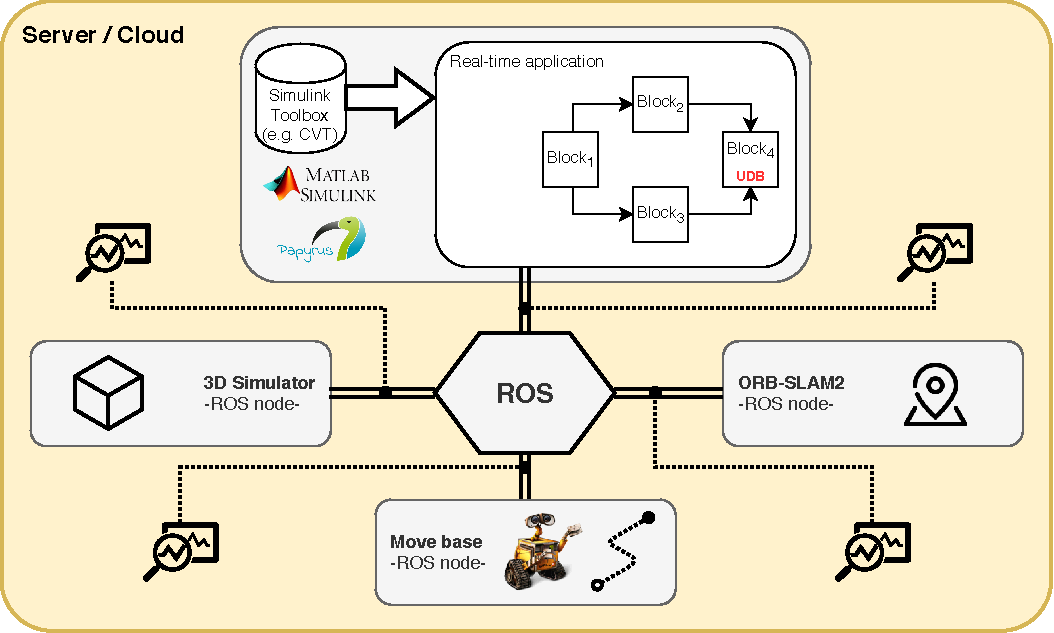
\includegraphics[width=\textwidth]{images/L1-arch}
	\caption{L1 architecture}
	\label{fig:l1arch}
\end{figure}

Because of the most used robotics platforms used today support the Melodic Morenia \cite{rosmelodic} version of ROS, and because of VOVD was written with the Kinetic version, it has been decided to convert VOVD in the relative Melodic ROS version. This task required a redefinition of some functions related to the ROS \textit{tf2} package \cite{tfros} due to the deprecation of the \textit{tf} package functions previously used. 
Another modification done talking about VOVD is related to the 3D map used by Gazebo \cite{Gazebo}. The problem was that it came with a featureless map generated from an URDF file, and because of ORB-SLAM2 properly works only if some features are detected during its execution, it has been necessary to add a material to the 3D model of the map.
Talking about ORB-SLAM2, it comes already provided with the necessaries functions to run in a ROS environment, thus no others operations have been required to complete our first architecture level.
%TODO a questo livello di architettura è possbile fare una verifica funzionale del sistema



\subsection{Architecture at L2} %TODO Work in progress
Another common architecture in robotics, involves the distribution of ROS nodes on different hadware platforms (e.g. NVIDIa Jetson or Raspberry). 
This step requires the split of our system in two parts: \textit{Host} (with Gazebo simulator) and \textit{Device/s} (robot navigation node/s). For this purpose, due to the several interconnected nodes, each of which having many parameters, it is raccomanded create a roslaunch file  using the \textit{machine tag}. These tags allow control over which nodes run on which machines, for load-balancing and bandwidth management. Fig. \ref{fig:l2arch} show an example of this confguration. At this architecture level the main focus is on the communication between the \textit{Host}, that act as Master, and the other external  nodes that rappresent the slaves. It is important to verify that the system continue working properly and that the Network doesn't become a bottleneck. For example, if we need to transfer a stream of images from one ROS nodes to another that is running on different machine, we should compress the images before send them over the netowork. In this way we avoid to saturate the bandwith of the network.

\begin{figure}
	\centering
	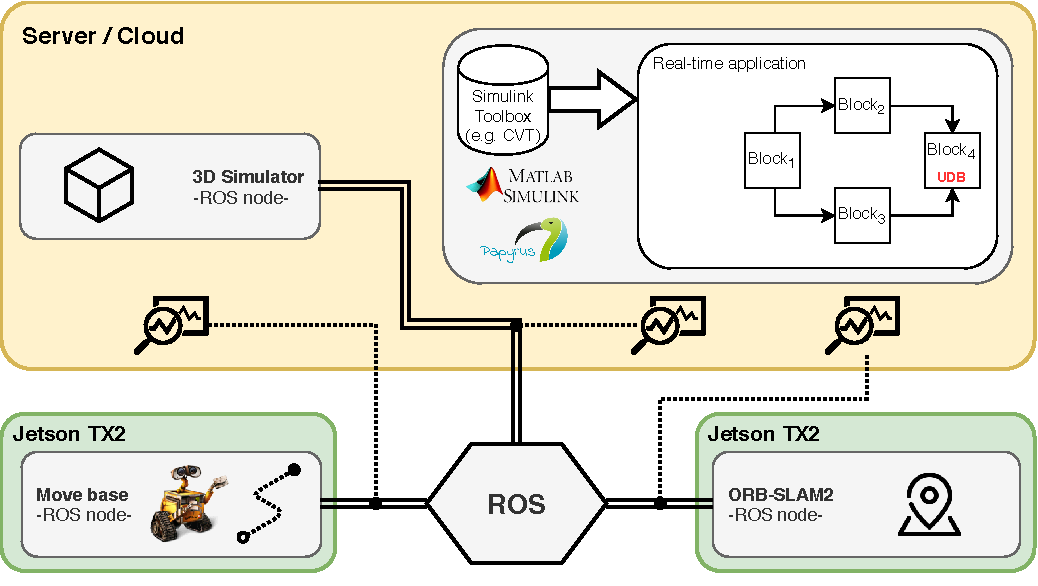
\includegraphics[width=\textwidth]{images/L2-arch}
	\caption{L2 architecture}
	\label{fig:l2arch}
\end{figure}




\subsection{Architecture at L3}	%TODO questo non lo abbiamo fatto ma lo mettiamo lo stesso.
Finally the last tipical architecture level is composed by \textit{Host}, \textit{Device/s } and  \textit{Robot/s}. If the previous step have been properly done, this one should be completely 
transparent with respect to the entire system. 
As we can see in Fig. \ref{fig:l3arch}, the simulator has been removed from the \textit{Host} and it is replaced by the real robot, on which one or more embedded devices are attached.
To achive this goal ... 
%TODO chiedere a piccinelli qual'è la modifica da fare per eseguire i comandi sul robot anziché sul simulatore


\begin{figure}
	\centering
	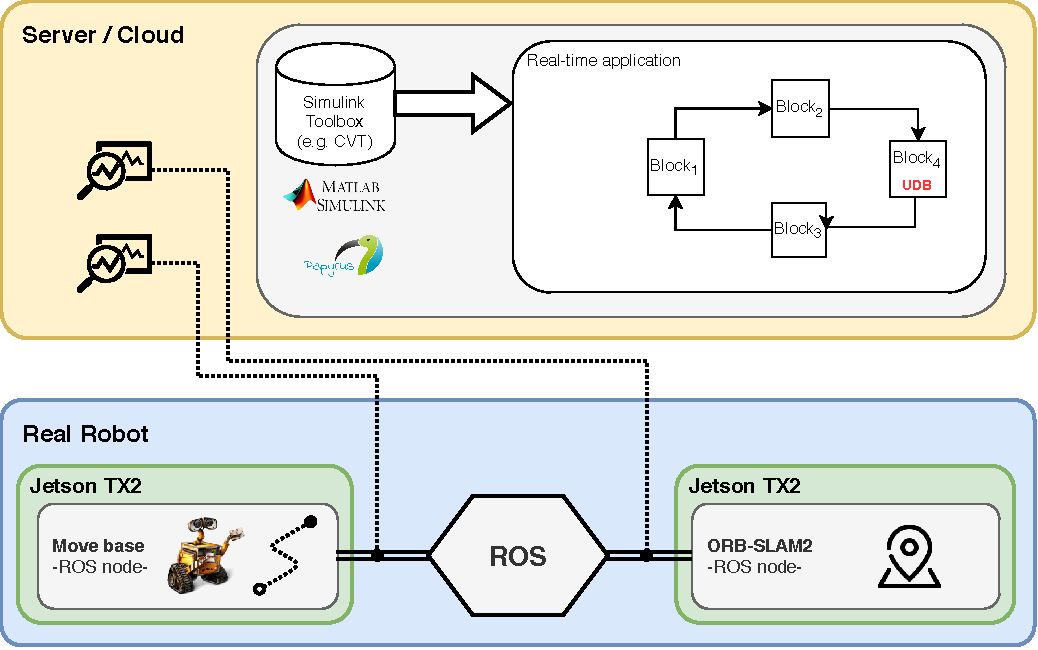
\includegraphics[width=\textwidth]{images/L3-arch}
	\caption{L3 architecture}
	\label{fig:l3arch}
\end{figure}


\section{Deployment from the cloud to the edge} % How to prepare an application for edge computing in Kubeedge?
As mentioned in \ref{kubeedgebackground}, Kubeedge is built upon Kubernetes and provides fundamental infrastructure support for network, app. deployment and metadata synchronization between cloud and edge. As we know, Kubernetes uses containers to run isolated, packaged applications across its cluster nodes. To run on Kubernetes, your applications must be encapsulated in one or more container images and executed using a container runtime like Docker. While containerizing your components is a requirement for Kubernetes, it also allow easy scaling and management. For instance, containers provide isolation between the application environment and the external host system, support a networked, service-oriented approach to inter-application communication, and typically take configuration through environmental variables and expose logs written to standard error and standard out. Containers themselves encourage process-based concurrency and help maintain dev/prod parity by being independently scalable and bundling the process’s runtime environment. These characteristics make it possible to package your applications so that they run smoothly on Kubernetes. In this section it will described the process used in our project to prepare both VOVD and ORB-SLAM2 applications for the edge computing through the support of Kubeedge.


\subsection{VOVD at the edge}
%TODO Dockerfile di VOVD 
%TODO Problemi in fase di building del container --> ROS network comunication


\subsection{ORB-SLAM2 at the edge}
%TODO Dockerfile di ORB_SLAM2 
%TODO Problemi in fase di building del container --> ROS + GPU (TRT)

\section{The whole system on Kubeedge}
%TODO Once we have containerized our applications we are ready to deploy them from the cloud to the edge with kubeedge: L1, L2, L3 ?!.



\section{Discussion}



\clearpage
\thispagestyle{empty}